\documentclass[a4paper,UTF8]{article}
\usepackage{amsmath}
\usepackage{amssymb}
\usepackage{amsthm}
\usepackage{bm}
\usepackage{color}
\usepackage{ctex}
\usepackage{enumerate}
\usepackage[margin=1.25in]{geometry}
\usepackage{graphicx}
\usepackage{hyperref}
\usepackage{tcolorbox}
\usepackage{algorithm}
\usepackage{algorithmic}
\theoremstyle{definition}
\newtheorem*{solution}{Solution}
\newtheorem*{prove}{Proof}
\newcommand{\indep}{\rotatebox[origin=c]{90}{$\models$}}

\usepackage{multirow}              

\setlength{\evensidemargin}{.25in}
\setlength{\textwidth}{6in}
\setlength{\topmargin}{-0.5in}
\setlength{\topmargin}{-0.5in}
% \setlength{\textheight}{9.5in}
%%%%%%%%%%%%%%%%%%此处用于设置页眉页脚%%%%%%%%%%%%%%%%%%
\usepackage{fancyhdr}                                
\usepackage{lastpage}                                           
\usepackage{layout}                                             
\footskip = 12pt 
\pagestyle{fancy}                    % 设置页眉                 
\lhead{2021年春季}                    
\chead{机器学习导论}                                                
% \rhead{第\thepage/\pageref{LastPage}页} 
\rhead{作业二}                                                                                               
\cfoot{\thepage}                                                
\renewcommand{\headrulewidth}{1pt}  			%页眉线宽,设为0可以去页眉线
\setlength{\skip\footins}{0.5cm}    			%脚注与正文的距离           
\renewcommand{\footrulewidth}{0pt}  			%页脚线宽,设为0可以去页脚线

\makeatletter 									%设置双线页眉                                        
\def\headrule{{\if@fancyplain\let\headrulewidth\plainheadrulewidth\fi%
		\hrule\@height 1.0pt \@width\headwidth\vskip1pt	%上面线为1pt粗  
		\hrule\@height 0.5pt\@width\headwidth  			%下面0.5pt粗            
		\vskip-2\headrulewidth\vskip-1pt}      			%两条线的距离1pt        
	\vspace{6mm}}     								%双线与下面正文之间的垂直间距              
\makeatother  


\begin{document}
\title{机器学习导论\\
	习题二}
\author{191300020, 黄彦骁, AdrianHuang@smail.nju.edu.cn}
\maketitle


\section*{学术诚信}

本课程非常重视学术诚信规范,助教老师和助教同学将不遗余力地维护作业中的学术诚信规范的建立。希望所有选课学生能够对此予以重视。\footnote{参考尹一通老师\href{http://tcs.nju.edu.cn/wiki/}{高级算法课程}中对学术诚信的说明。}

\begin{tcolorbox}
	\begin{enumerate}[(1)]
		\item 允许同学之间的相互讨论,但是{\color{red}\textbf{署你名字的工作必须由你完成}},不允许直接照搬任何已有的材料,必须独立完成作业的书写过程;
		\item 在完成作业过程中,对他人工作(出版物、互联网资料)中文本的直接照搬(包括原文的直接复制粘贴及语句的简单修改等)都将视为剽窃,剽窃者成绩将被取消。{\color{red}\textbf{对于完成作业中有关键作用的公开资料,应予以明显引用}};
		\item 如果发现作业之间高度相似将被判定为互相抄袭行为,{\color{red}\textbf{抄袭和被抄袭双方的成绩都将被取消}}。因此请主动防止自己的作业被他人抄袭。
	\end{enumerate}
\end{tcolorbox}

\section*{作业提交注意事项}
\begin{tcolorbox}
	\begin{enumerate}[(1)]
		\item 请在{\color{red}\textbf{第一页填写个人的姓名、学号、邮箱信息}};
		\item 本次作业需提交该pdf文件,pdf文件名格式为{\color{red}\textbf{学号\_姓名.pdf}},例如190000001\_张三.pdf,{\color{red}\textbf{需通过教学立方提交}}。
		\item 未按照要求提交作业,或提交作业格式不正确,将会{\color{red}\textbf{被扣除部分作业分数}};
		\item 本次作业提交截止时间为{\color{red}\textbf{4月16日23:55:00。}}
	\end{enumerate}
\end{tcolorbox}

\newpage

\section{[40pts] Linear Discriminant Analysis}
课本中介绍的 Fisher 判别分析 (Fisher Discriminant Analysis, FDA) 没有对样本分布进行假设. 当假设各类样本的协方差矩阵相同时, FDA 退化为线性判别分析 (Linear Discriminant Analysis, LDA). 考虑一般的$K$分类问题, $\left\{(\bm{x}_1,y_1),(\bm{x}_2,y_2),\cdots,(\bm{x}_m,y_m)\right\}$为训练集, 其中, 第 $k$ 类样本从正态分布 $\mathcal{N}(\bm{\mu}_k,\bm{\Sigma})$ 中独立同分布采样得到 ($k=1,2,\cdots,K$, 各类共享协方差矩阵), 记该类样本数量为 $m_k$, 类概率 $\Pr\left(y=k\right)=\pi_k$. 若 $X\in \mathbb{R}^d \sim \mathcal{N}(\bm{\mu},\bm{\Sigma})$, 则其概率密度函数为
\begin{align}
	p(x)=\frac{1}{(2\pi)^{\frac{d}{2}}\det\left(\bm{\Sigma}\right)^\frac{1}{2}}\exp\left(-\frac{1}{2}(\bm{x}-\bm{\mu})^T\bm{\Sigma}^{-1}(\bm{x}-\bm{\mu})\right).
\end{align}
请回答下列问题:

\begin{enumerate}[(1)]
	\item \textbf{[6pts]} (贝叶斯最优分类器) \label{Q1q1}从贝叶斯决策论的角度出发, 对样本 $\bm{x}$ 做出的最优预测应为 $\arg\max_y$ $\Pr\left(y\mid \bm{x}\right)$. 因此, 只需考察 $\ln\Pr(y=k\mid \bm{x})$的大小, 即可得到贝叶斯最优分类器, 这也正是推导LDA的一种思路. 请证明: 在题给假设下, $\arg\max_y \Pr\left(y\mid \bm{x}\right)=\arg\max_k \delta_k(\bm{x})$, 其中 $\delta_{k}(\bm{x})=\bm{x}^{T} \bm{\Sigma}^{-1} \bm{\mu}_{k}-\frac{1}{2} \bm{\mu}_{k}^{T} \bm{\Sigma}^{-1} \bm{\mu}_{k}+\ln \pi_{k}$ 为LDA在分类时的判别式.
	\item \textbf{[6pts]} \label{Q1q2} 假设 $K=2$, 记 $\hat{\pi}_{k}=\frac{m_k}{m}$, $\hat{\bm{\mu}}_{k}=\frac{1}{m_k}\sum_{y_{i}=k} \bm{x}_{i}$, $\hat{\bm{\Sigma}}=\frac{1}{m-K}\sum_{k=1}^{K} \sum_{y_{i}=k}$ $\left(\bm{x}_{i}-\hat{\bm{\mu}}_{k}\right)$ $\left(\bm{x}_{i}-\hat{\bm{\mu}}_{k}\right)^{T}$. LDA使用这些经验量替代真实参数, 计算判别式 $\delta_k(\bm{x})$ 并按照第(\ref{Q1q1})问中的准则做出预测. 请证明: 在 $\bm{x}^{T} \hat{\bm{\Sigma}}^{-1}\left(\hat{\bm{\mu}}_{2}-\hat{\bm{\mu}}_{1}\right)>\frac{1}{2}\left(\hat{\bm{\mu}}_{2}+\hat{\bm{\mu}}_{1}\right)^{T} \hat{\bm{\Sigma}}^{-1}\left(\hat{\bm{\mu}}_{2}-\hat{\bm{\mu}}_{1}\right)-\ln \left(m_{2} / m_{1}\right)$ 时 LDA 将样本预测为第 2 类.
	\item \textbf{[16pts]} (线性回归) 考虑第(\ref{Q1q2})问中的二分类问题, 并将第 1 类样本的标记 $y$ 设为 $-\frac{m}{m_1}$, 将第 2 类样本的标记 $y$ 设为 $\frac{m}{m_2}$. 仿照线性回归, 得到下列优化问题:
	      \begin{align}
		      \label{ols}
		      \min_{\bm{\beta},\beta_0} \quad \sum_{i=1}^m(y_i-\beta_0-\bm{x}_i^T\bm{\beta})^2.
	      \end{align}
	      请证明: 上述优化问题的最优解满足 $\bm{\beta}^*\propto \hat{\bm{\Sigma}}^{-1}\left(\hat{\bm{\mu}}_{2}-\hat{\bm{\mu}}_{1}\right)$, 即通过线性回归解得的 $\bm{x}$ 系数与第(\ref{Q1q2})问中LDA的判别规则表达式中的 $\bm{x}$ 系数同向.
	\item \textbf{[6pts]} (对率回归) 通过课本的介绍可知对率回归假设对数几率为特征 $\bm{x}$ 的线性函数, 而由第(\ref{Q1q1})问可知, 在LDA 中, 对数几率 $\ln\frac{\Pr(y=k|\bm{x})}{\Pr(y=l|\bm{x})}$ 也可以写成 $\beta_0+\bm{x}^T\bm{\beta}$ 的形式, 从这一角度来看, 这两种模型似乎是相同的? 哪种模型做出的假设更强? 请说明理由.
	\item \textbf{[6pts]} (二次判别分析) 假设各类样本仍服从正态分布, 但第 $k$ 类样本从 $\mathcal{N}(\bm{\mu}_k,\bm{\Sigma}_k)$ 中独立同分布采样得到, 即不假设各类的协方差矩阵相同. 请按照第(\ref{Q1q1})问中的思路, 给出分类应采用的判别式 $\delta_k(\bm{x})$, 使得 $\arg\max_y \Pr\left(y\mid \bm{x}\right)=\arg\max_k \delta_k(\bm{x})$. 此时判别式是一个关于$\bm{x}$的二次函数, 这一做法被称为二次判别分析 (Quadratic Discriminant Analysis, QDA).
\end{enumerate}

\begin{solution}
	\begin{enumerate}
		\item [(1)]
		      \begin{align*}
			      \arg \max_y \Pr(y\mid \bm{x}) & = \arg \max_y \ln \Pr(y=k\mid x)                                                                                                                                                                                                          \\
			                                    & = \arg \max_k \ln \frac{P(X = x | Y = k)*P(Y=k)}{P(X = x)}                                                                                                                                                                                \\
			                                    & = \arg \max_k \ln \frac{P_{k}(x) \cdot \pi_{k}}{P(X=x)}                                                                                                                                                                                   \\
			                                    & = \arg \max_k \ln P_{k}(x) \cdot \pi_{k}                                                                                                                                                                                                  \\
			                                    & = \arg \max_k \ln \frac{1}{(2 \pi)^{\frac{d}{2}} \det(\bm{\Sigma})^{\frac{1}{2}}}-\frac{1}{2}\left(\boldsymbol{x}-\boldsymbol{\mu}_{k}\right)^{\top} \boldsymbol{\Sigma}^{-1}\left(\boldsymbol{x}-\boldsymbol{\mu}_{k}\right)+\ln \pi_{k} \\
			                                    & = \arg \max_k \boldsymbol{x}^{T} \boldsymbol{\Sigma}^{-1} \boldsymbol{\mu}_{k}-\frac{1}{2} \boldsymbol{\mu}_{k}^{T} \boldsymbol{\Sigma}^{-1} \boldsymbol{\mu}_{k}+\ln \pi_{k}                                                             \\
			                                    & = \arg \max_k \delta_k(\bm{x})                                                                                                                                                                                                            \\
		      \end{align*}
		\item [(2)]
		      要说明$LDA$将样本预测为第2类,即只需说明$\delta_2(\bm{x})> \delta_1(\bm{x})$即可:
		      \begin{align*}
			      \delta_2(\bm{x})> \delta_1(\bm{x}) & = \boldsymbol{x}^{\top} \hat{\bm{\Sigma}}^{-1} \hat{\boldsymbol{\mu}}_{2}-\frac{1}{2} \hat{\boldsymbol{\mu}}_{2}^{\top} \hat{\bm{\Sigma}}^{-1} \hat{\boldsymbol{\mu}}_{2}+\ln \pi_{2}-\boldsymbol{x}^{\top} \hat{\bm{\Sigma}}^{-1} \hat{\boldsymbol{\mu}}_{1}+\frac{1}{2} \hat{\boldsymbol{\mu}}_{1}^{\top} \hat{\bm{\Sigma}}^{-1} \hat{\boldsymbol{\mu}}_{1}-\ln \pi_{1} \\
			                                         & = \bm{x}^{T} \hat{\bm{\Sigma}}^{-1}\left(\hat{\bm{\mu}}_{2}-\hat{\bm{\mu}}_{1}\right)>\frac{1}{2}\left(\hat{\bm{\mu}}_{2}+\hat{\bm{\mu}}_{1}\right)^{T} \hat{\bm{\Sigma}}^{-1}\left(\hat{\bm{\mu}}_{2}-\hat{\bm{\mu}}_{1}\right)-\ln \left(m_{2} / m_{1}\right)                                                                                                           \\
			                                         & > 0                                                                                                                                                                                                                                                                                                                                                                       \\
		      \end{align*}
		      故可以证得。
		\item [(3)]
		      令$f=\sum_{i=1}^m(y_i-\beta_0-\bm{x}_i^T\bm{\beta})^2$,对其求偏导得:
		      \[\frac{\partial f}{\partial \beta_{0}}= - 2 \sum_{i=1}^{m}\left(y_{i}-\beta_{0}-\boldsymbol{x}_{i}^{\top} \boldsymbol{\beta}\right)\]
		      \[\frac{\partial f}{\partial \boldsymbol{\beta}}=-2 \sum_{i=1}^{m}\left(y_{i}-\beta_{0}-\boldsymbol{x}_{i}^{\top} \boldsymbol{\beta}\right)^{\top} \boldsymbol{x}_{i}^{\top}\]
		      为求其最优解,令其偏导等于零可得:
		      \[\beta_0= \frac{1}{m}\sum_{i=1}^m(y_i-\bm{x}_i^T\bm{\beta})^2\]
		      由于$\sum_{i=1}^my_i=m_1*(-\frac{m}{m_1})+m_2 * \frac{m}{m_2}=0$,所以有:
		      \[\beta_0=-\frac{m_1\hat{\bm{\mu_1}}+m_2\hat{\bm{\mu}}_2}{m}\bm{\beta}=-\hat{\bm{\mu}}\bm{\beta}\]
		      代入原式得:
		      \begin{align*}
			      f & = \sum_{i=1}^{m}\left(y_{i}-\left(\hat{\boldsymbol{\mu}}^{\top}+\boldsymbol{x}_{i}^{\top}\right) \boldsymbol{\beta}\right)^{2}       \\
			        & = \sum_{i=1}^m(y_i^2-2y_i(\hat{\bm{\mu}}^{\top}+\bm{x}_i^{\top})\bm{\beta}+((\hat{\bm{\mu}}^{\top}+\bm{x}_i^{\top})\bm{\beta})^2)    \\
			        & = (\frac{1}{m_1}+\frac{1}{m_2})m^2-2m(\hat{\bm{\mu}}_2-\hat{\bm{\mu}_1})\bm{\beta}+(m-2)\bm{\beta}^{\top}\hat{\bm{\Sigma}}\bm{\beta} \\
		      \end{align*}
		      对$\bm{\beta}$求导得:
		      \[\frac{\partial f}{\partial \bm{\beta}}=2(m-2)\hat{\bm{\Sigma}}\bm{\beta}-2m(\hat{\bm{\mu}}_2-\hat{\bm{\mu}}_1)\]
		      令其等于可以得到:
		      \[\bm{\beta}=\frac{m}{m-2}\hat{\bm{\Sigma}}^{-1}(\hat{\bm{\mu}}_2-\hat{\bm{\mu}}_1)\]
		      所以有$\beta^{*} \propto \hat{\Sigma}^{-1}\left(\hat{\mu}^{1}-\hat{\mu}_{2}\right)$.
		\item [(4)]
		      我认为是LDA模型更强,对数几率回归中是对$y$进行了类后验概率$p(y=i|x)$的假设,而LDA中需要我们对理论参数进行估计,用样本参量代入理论模型来进行模拟,样本在估计时的参与率更高。
		\item [(5)]
		      与第一题类似:
		      \begin{align*}
			      \arg \max_y \Pr(y\mid \bm{x}) & = \arg \max_y \ln \Pr(y=k\mid x)                                                                                                                                                                                                          \\
			                                    & = \arg \max_k \ln \frac{P(X = x | Y = k)*P(Y=k)}{P(X = x)}                                                                                                                                                                                \\
			                                    & = \arg \max_k \ln \frac{P_{k}(x) \cdot \pi_{k}}{P(X=x)}                                                                                                                                                                                   \\
			                                    & = \arg \max_k \ln P_{k}(x) \cdot \pi_{k}                                                                                                                                                                                                  \\
			                                    & = \arg \max_k \ln \frac{1}{(2 \pi)^{\frac{d}{2}} \det(\bm{\Sigma})^{\frac{1}{2}}}-\frac{1}{2}\left(\boldsymbol{x}-\boldsymbol{\mu}_{k}\right)^{\top} \boldsymbol{\Sigma}^{-1}\left(\boldsymbol{x}-\boldsymbol{\mu}_{k}\right)+\ln \pi_{k} \\
			                                    & = \arg \max_k -\frac{1}{2}\ln (|\bm{\Sigma}|_2^2)+ \boldsymbol{x}^{T} \boldsymbol{\Sigma}^{-1} \boldsymbol{\mu}_{k}-\frac{1}{2} \boldsymbol{\mu}_{k}^{T} \boldsymbol{\Sigma}^{-1} \boldsymbol{\mu}_{k}+\ln \pi_{k}                        \\
		      \end{align*}
		      即可得到。
	\end{enumerate}
\end{solution}

\section{[30pts] Generalized Rayleigh Quotient}
在面对多类样本时, FDA 需要求解广义瑞利商:
\begin{align}
	\label{fda}
	\max_{\bm{w}}\quad\frac{\bm{w}^T\bm{S}_b\bm{w}}{\bm{w}^T\bm{S}_w\bm{w}}.
\end{align}
\begin{enumerate}[(1)]
	\item \textbf{[15pts]} 请证明: 瑞利商满足
	      \begin{align}
		      \lambda_{\text{min}}(\bm{A})\le \frac{\bm{w}^T\bm{A}\bm{w}}{\bm{w}^T\bm{w}}\le \lambda_{\text{max}}(\bm{A}),
	      \end{align}
	      其中 $\bm{A}$ 为实对称矩阵, $\lambda(\bm{A})$ 为 $\bm{A}$ 的特征值.
	\item \textbf{[15pts]} 请证明: 如果 $\bm{A}$ 为实对称矩阵, $\bm{B}$ 为正定矩阵, 那么广义瑞利商满足
	      \begin{align}
		      \lambda_{\text{min}}(\bm{B}^{-1}\bm{A})\le \frac{\bm{w}^T\bm{A}\bm{w}}{\bm{w}^T\bm{B}\bm{w}}\le \lambda_{\text{max}}(\bm{B}^{-1}\bm{A}).
	      \end{align}
\end{enumerate}

\begin{solution}
	\begin{enumerate}
		\item [(1)]
		      由于$A$为实对称矩阵,不妨设其维度为$n$,设其特征值为$\lambda_1,\lambda_2\ldots\lambda_n$同时有:
		      \[\lambda_{min}\leqslant \lambda_1\leqslant\lambda_2\leqslant\ldots\leqslant\lambda_n\leqslant\lambda_{max}\]
		      所以存在正定矩阵使得$\bm{U}$和对角矩阵$\bm{M}$使得$\bm{A}=\bm{U}\bm{M}\bm{U}^T$,其中$M=diag(\lambda_1, \lambda_2, \ldots, \lambda_n)$,
		      将上式代入瑞利商得:
		      \[\frac{\bm{w}^T\bm{A}\bm{w}}{\bm{w}^T\bm{w}}=\frac{(\bm{U}^T\bm{w})^T\bm{M}(\bm{U}^T\bm{w})}{\bm{w}^T\bm{w}}\]
		      设$\bm{p}=\bm{U}^T\bm{w}$,同时$p_i$为$\bm{p}$的第$i$个元素,那么上式即可写为:
		      \[\frac{\bm{p}^T\bm{M}\bm{p}}{\bm{w}^T\bm{w}}=\frac{\sum_{i=1}^n\lambda_i|p_i|^2}{\sum_{i=1}^n|w_i|^2}\]
		      由特征值的大小关系有:
		      \[\frac{\lambda_1\sum_{i=1}^n|p_i|^2}{\sum_{i=1}^n|w_i|^2}\leqslant \frac{\sum_{i=1}^n\lambda_i|p_i|^2}{\sum_{i=1}^n|w_i|^2}\leqslant \frac{\lambda_n\sum_{i=1}^n|p_i|^2}{\sum_{i=1}^n|w_i|^2}\]
		      设$\bm{U}$的第$i$行第$j$列的元素为$u_{ij}$,那么:
		      \[p_i=\sum_{j=1}^nu_{ij}x_j, p_i^T=\sum_{j=1}^nx_ju_{ij}\]
		      \[|p_{i}|^{2}=p_{i}^{T} p_{i}=\sum_{j=1}^{n} \sum_{k=1}^{n} x_{j} u_{i j} u_{k i} x_{k}\]
		      于是有:
		      \[\sum_{i=1}^{n}\left|p_{i}\right|^{2}=\sum_{j=1}^{n} \sum_{k=1}^{n}\left(\sum_{i=1}^{n} u_{k i} u_{i j}\right) x_{j} x_{k}\]
		      由$\bm{U}$为正定矩阵有$\bm{U}^T\bm{U}=\bm{I}$,那么上式即可等价为:
		      \[I_{j k}=\sum_{i=1}^{n} u_{j i} u_{i k}\]
		      当$j=k$时,$I_{jk}=1$,否则$I_{jk}=0$,所以得到:
		      \[\sum_{i=1}^{n}\left|p_{i}\right|^{2}=\sum_{i=1}^{n}\left|x_{i}\right|^{2}\]
		      将上述代入原式得:
		      \[\lambda_{\min }(\bm{A}) \leq \frac{\bm{w}^{T} \bm{A} \bm{w}}{\bm{w}^{T} \bm{w}} \leq \lambda_{\max }(\bm{A})\]
		\item [(2)]
		      我们不妨令$\bm{w}=\bm{B}^{-\frac{1}{2}}\bm{w}_1$,那么便有:
		      \[\frac{\bm{w}^{T} \bm{A} \bm{w}}{\bm{w}^{T} \bm{B} \bm{w}}= \frac{\bm{w}^T\bm{B}^{-\frac{1}{2}}\bm{A}\bm{B}^{-\frac{1}{2}}\bm{w}}{\bm{w}_1^T\bm{w}_1}\]
		      所以有:
		      \[\lambda_{min}(\bm{B}^{-\frac{1}{2}}\bm{A}\bm{B}^{-\frac{1}{2}})\leq \frac{\bm{w}^T \bm{A} \bm{w}}{\bm{w}^T \bm{B} \bm{w}}\leq\lambda_{max}(\bm{B}^{-\frac{1}{2}}\bm{A}\bm{B}^{-\frac{1}{2}})\]
		      而由于$(\bm{B}^{-\frac{1}{2}}\bm{A}\bm{B}^{-\frac{1}{2}})^T=(\bm{B}^{-\frac{1}{2}})^T(\bm{A}\bm{B}^{-\frac{1}{2}})^T=\bm{B}^{-\frac{1}{2}}\bm{B}^{-\frac{1}{2}}\bm{A}=\bm{B}^{-1}\bm{A}$
		      所以$\bm{B}^{-\frac{1}{2}}\bm{A}\bm{B}^{-\frac{1}{2}}$与$\bm{B}^{-1}\bm{A}$特征值相等,所以有:
		      \[\lambda_{min}(\bm{B}^{-1}\bm{A})\leq\frac{\bm{w}^{T} \bm{A} \bm{w}}{\bm{w}^{T} \bm{B} \bm{w}}\leq\lambda_{max}(\bm{B}^{-1}\bm{A})\]
	\end{enumerate}
\end{solution}

\section{[30+10*pts] Decision Tree}

\begin{enumerate}[(1)]
	\item \textbf{[15pts]} 对于不含冲突样本 (即特征相同但标记不同) 的训练集, 必存在与训练集一致 (即训练误差为 0) 的决策树. 如果训练集可以包含无穷多个样本, 是否一定存在与训练集一致的深度有限的决策树? 证明你的结论. (仅考虑单个划分准则仅包含一次属性判断的决策树)
	\item \textbf{[15pts]} 考虑如表\ref{data}所示的人造数据, 其中“性别”、“喜欢ML作业”是特征, “ML成绩高”是标记. 请画出\textbf{所有}可能的使用信息增益为划分准则产生的决策树. (不需要写出计算过程)
	      \begin{table}[h]
		      \caption{人造训练集}
		      \label{data}
		      \centering
		      \begin{tabular}{cccc}
			      \hline
			      编号 & 性别 & 喜欢ML作业 & ML成绩高 \\
			      \hline
			      1    & 男   & 是         & 是       \\
			      2    & 女   & 是         & 是       \\
			      3    & 男   & 否         & 否       \\
			      4    & 男   & 否         & 否       \\
			      5    & 女   & 否         & 是       \\
			      \hline
		      \end{tabular}
	      \end{table}
	\item \textbf{[10*pts]} 在决策树的生成过程中, 需要计算信息增益以生成新的结点. 设 $a$ 为有$V$个可能取值$\left\{a^1,a^2,\cdots,a^V\right\}$的离散属性, 请证明:
	      \begin{align}
		      \text{Gain}(D,a)=\text{Ent}(D)-\sum_{v=1}^V\frac{\lvert D^v\rvert}{\lvert D\rvert}\text{Ent}(D^v)\ge 0,
	      \end{align}
	      即信息增益非负.
\end{enumerate}

\begin{solution}
	\begin{enumerate}
		\item [(1)]
		      不一定,考虑数据集$\left\{(\frac{1}{i}, (-1)^i)\right\}_{i=1}^{\infty}$。
		      若决策树为有限深度,那么其只能进行有限次属性判断,区间只能被划分为有限个区域,但该数据集将区间划分为无穷多个区域。
		\item [(2)]
		      \begin{figure}
			      \centering
			      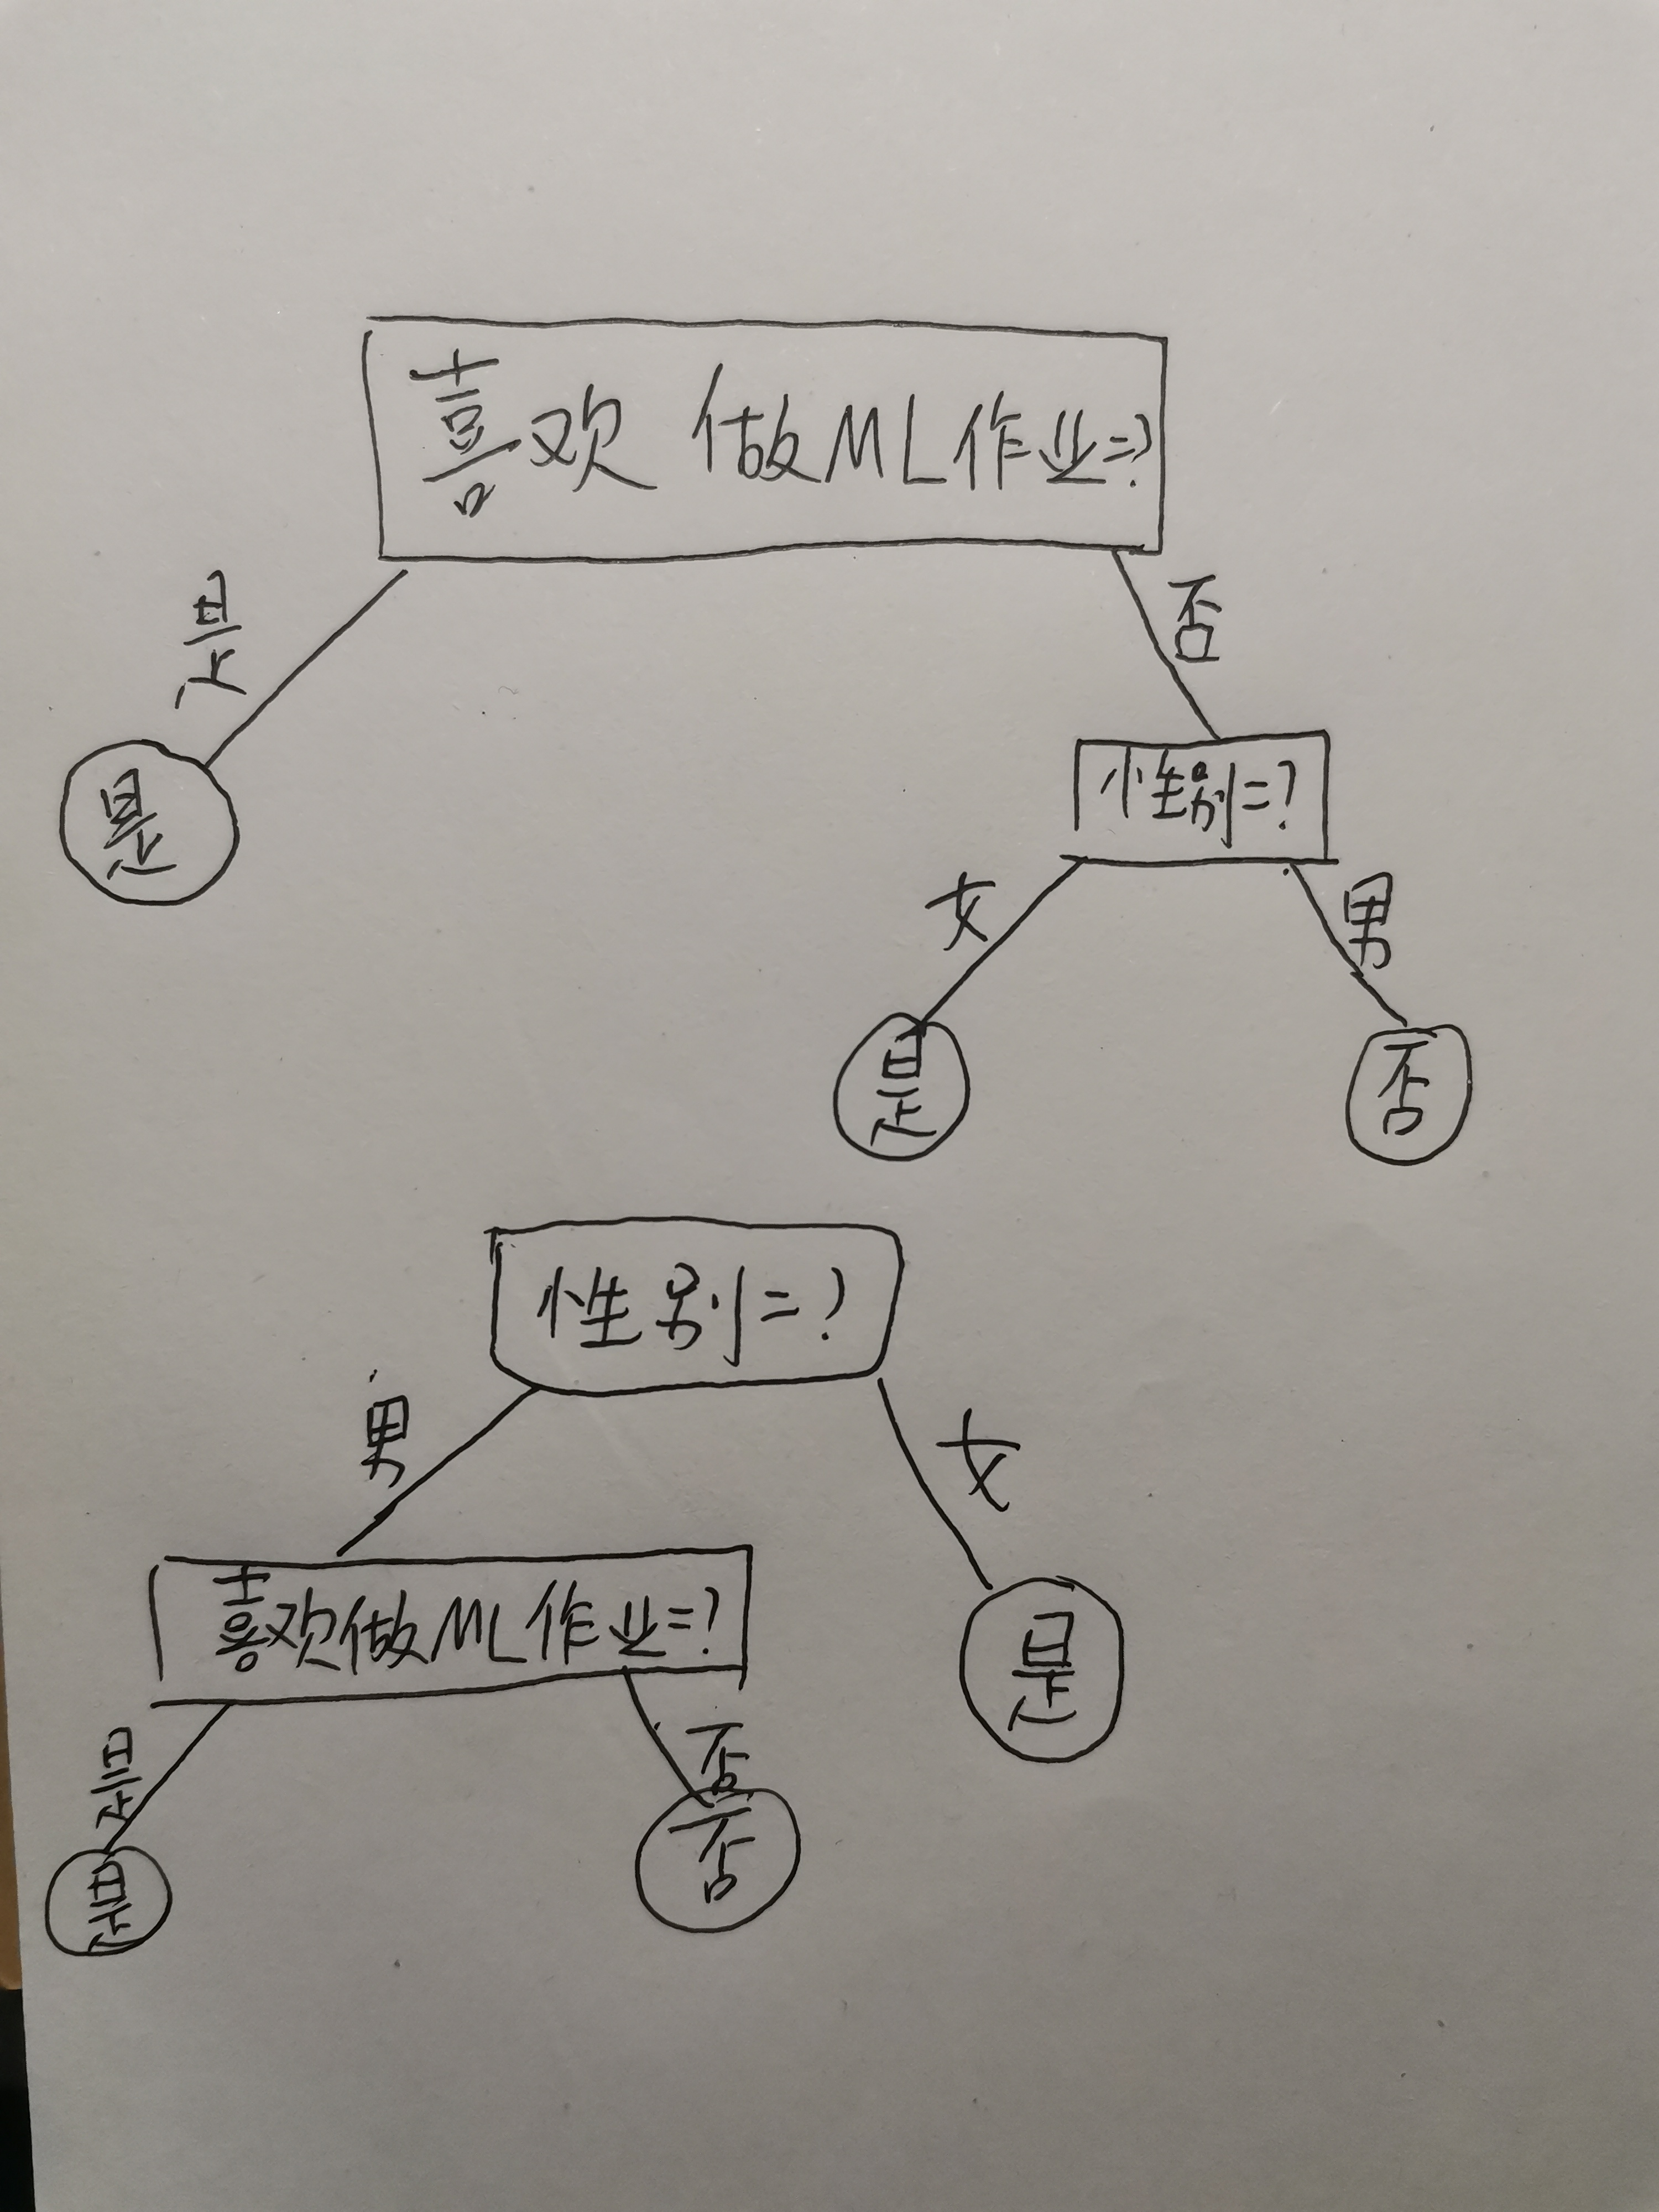
\includegraphics[width=5cm,height=7cm]{P3-2.jpg}
			      \caption{决策树结果}
		      \end{figure}
		      结果见图1
		\item [(3)]
		      我们不妨设$P(X)$为第$X$个标记样本占总体的比例,$P(K)$为第$K$个可能取值样本占总体的比例,$P(X,K)$为第$K$个可能取值样本中标记为$X$的样本占总体的比例
		      有$P(X|K) = \frac{P(X,K)}{P(K)},P(X)=\sum_KP(X,K),P(K)=\sum_XP(X,K)$。
		      \begin{proof}
			      \begin{align*}
				      Gain(D,a)  & = \sum_{X}-P(X) \log _{2} P(X)-\sum_{K} P(K) \sum_{X}\left(-P(X \mid K) \log _{2} P(X \mid K)\right)                         \\
				      -Gaim(D,a) & = \sum_{X} P(X) \log _{2} P(X)-\sum_{K} P(K) \sum_{X}\left(P(X \mid K) \log _{2} P(X \mid K)\right)                          \\
				                 & = \sum_{X} P(X) \log _{2} P(X)-\sum_{K} P(K) \sum_{X}\left(P(X \mid K) \log _{2} P(X \mid K)\right)                          \\
				                 & = \sum_{X} \sum_{K} P(X, K) \log _{2} P(X)-\sum_{K} \sum_{X}\left(P(K) P(X \mid K) \log _{2} P(X \mid K)\right)              \\
				                 & = \sum_{X} \sum_{K} P(X, K) \log _{2} P(X)-\sum_{K} \sum_{X}\left(P(X, K) \log _{2} P(X \mid K)\right)                       \\
				                 & = \sum_{X} \sum_{K} P(X, K)\left(\log _{2} P(X)-\log _{2} P(X \mid K)\right)                                                 \\
				                 & = \sum_{X} \sum_{K} P(X, K)\left(\log _{2}\left(\frac{P(X)}{P(X \mid K)}\right)\right)                                       \\
				                 & = \sum_{X} \sum_{K} P(X \mid K) P(K)\left(\log _{2}\left(\frac{P(X)}{P(X \mid K)}\right)\right)                              \\
				                 & = \sum_{K} P(K) \sum_{X} P(X \mid K)\left(\log _{2}\left(\frac{P(X)}{P(X \mid K)}\right)\right)                              \\
				                 & \leq \sum_{K} P(K)\left(\log _{2}\left(\sum_{X} \frac{P(X \mid K) P(X)}{P(X \mid K)}\right)\right)(From\ Jensen\ Inequality) \\
				                 & \leq \log _{2}\left(\sum_{K} \sum_{X} \frac{P(K) P(X \mid K) P(X)}{P(X \mid K)}\right) (From\ Jensen\ Inequality)            \\
				                 & \leq \log _{2}\left(\sum_{K} \sum_{X} P(K) P(X)\right)                                                                       \\
				                 & \leq \log _{2}\left(\sum_{K} P(K) \sum_{X} P(X)\right)                                                                       \\
				                 & \leq \log _{2}\left(\sum_{K} P(K)\right)                                                                                     \\
				                 & \leq \log _{2}(1)                                                                                                            \\
				                 & \leq 0
			      \end{align*}
		      \end{proof}
		      所以有$Gaim(D,a)\geqslant 0$.
	\end{enumerate}
\end{solution}

\end{document}